\documentclass[a4paper,12pt,openany]{article}

\usepackage[brazil]{babel}
\usepackage[T1]{fontenc}
\usepackage{ae}
\usepackage[utf8]{inputenc}
\usepackage{graphicx}
\usepackage{indentfirst}
\usepackage{amstext}
\usepackage{amssymb}
\usepackage[a4paper,left=3cm,right=3cm,top=3cm,bottom=3cm]{geometry}
\usepackage{tipa}
\usepackage[colorlinks,breaklinks,urlcolor=blue,linkcolor=black]{hyperref}
\usepackage{setspace}
\usepackage{color}
\usepackage{multirow}


%############ BACKGROUND ##################
\usepackage{eso-pic}
\newcommand\BackgroundPic{
\put(0,0){
\parbox[b][\paperheight]{\paperwidth}{
\vfill
\centering
%\includegraphics[width=.95\paperwidth,height=.95\paperheight,keepaspectratio]{o-grito.jpg}
%\includegraphics[width=.9\paperwidth,height=.9\paperheight,keepaspectratio]{o_grito_moderno.jpg}
%\includegraphics[width=.9\paperwidth,height=.9\paperheight,keepaspectratio]{Grito_PB.jpg}
\vfill
}}}

%############### FONTE #####################
\usepackage[T1]{fontenc}
%\usepackage[lf]{venturis} %% lf option gives lining figures as default;
% remove option to get oldstyle figures as default
%\renewcommand*\familydefault{\sfdefault} %% Only if the base font of the document is to be sans serif

%############### Ordinais ##################
\newcommand{\ORD}{\raise1ex\hbox{\underbar{\scriptsize o}}}


\begin{document}

	\begin{titlepage}
	
	%\AddToShipoutPicture*{\BackgroundPic}

        \begin{center}
            UNIVERSIDADE TECNOLÓGICA FEDERAL DO PARANÁ\\
            DEPARTAMENTO ACADÊMICO DE INFORMÁTICA\\
            CAMPUS CURITIBA

            \vspace{4cm}

            PET-ECO APRESENTA

            \vfill

           % {\Huge \emph{\colorbox{black}{\color{red} NÃO ENTRE EM PÂNICO!}} }
	        { \Huge \emph { \textbf {NÃO ENTRE EM PÂNICO! }} }

          	%\includegraphics[width=.7\linewidth]{o_grito_moderno.jpg}

            \vspace{4cm}

           % {\LARGE \textbf{\color{blue} MANUAL DE SOBREVIVÊNCIA} }
	        { \LARGE \textbf {Manual de Sobrevivência} }

            \vfill

            2011
        \end{center}

	\end{titlepage}

% ************************* SUMÁRIO *******************************************
\thispagestyle{empty}
\tableofcontents

% *********************** INTRODUÇÃO ******************************************
\newpage
\section{Introdução}

Bem-vindo à Universidade Tecnológica Federal do Paraná! Nossos cumprimentos por esta conquista. Você está dando um dos passos mais importantes de sua vida: escolher uma carreira.

Mas, se você está totalmente perdido, não se desespere! Felizmente, você não é o primeiro e nem será o último a viver essa situação. Então, respire fundo, conte até dez e leia até o fim deste manual (se não dormir antes). Ele contem informações e dicas importantes para sobreviver a esse universo novo chamado Universidade Tecnológica Federal do Paraná.  

Elaborado pelos integrantes do grupo PET de Engenharia de Computação, este manual foi feito ajudar a esclarecer algumas dúvidas que são comuns entre os calouros. Caso ainda se sinta confuso com relação a alguma coisa, fique à vontade para procurar o PET-ECO (nos corredores ou \url{http://www.dainf.ct.utfpr.edu.br/peteco} ou ainda \href{mailto:petecoutfpr@gmail.com}{petecoutfpr@gmail.com}) e esclarecer suas dúvidas ou sugerir modificações no texto.


	\begin{figure}[ht!]  \centering
		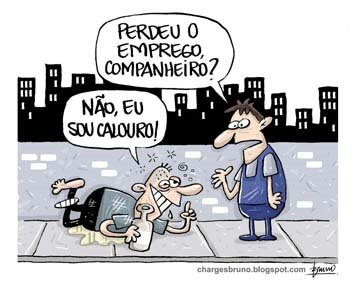
\includegraphics[scale=1]{calouro.jpg}
		\caption{Com esse manual, esperamos evitar que você passe por esta situação.}
		\label{fig01}
	\end{figure}

	

% *********************** LOCALIZE-SE *****************************************
\newpage
\section{Localize-se!}

A Sede Central do Campus Curitiba da UTFPR é relativamente pequena, pois ocupa apenas uma quadra. Apesar disso, no começo, é comum não encontrar alguns lugares aonde se deseja ir. Logo você se acostuma!

%    \begin{figure}[ht!]  \centering
%		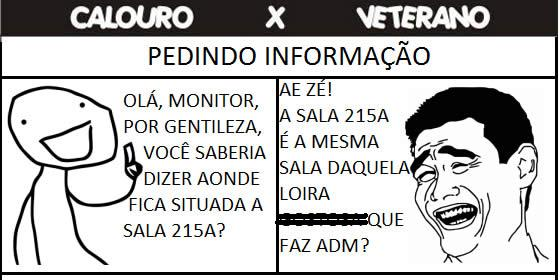
\includegraphics[scale=0.5]{calouro1.jpg}
%		%\caption{Calouro}
%		\label{fig02}
%	\end{figure}

Incluímos neste mapa resumido alguns lugares que consideramos importantes para os calouros do DAINF. São eles:

	\begin{figure}[ht!]  \centering
		\includegraphics[scale=0.7]{mapa.png}
		\caption{Mapa do Campus Curitiba Centro}
		\label{fig03}
	\end{figure}


\begin{itemize}

\item \textbf{Auditório e Miniauditório} (Bloco H e J)\\ aqui acontecem diversos eventos durante o semestre.

\item \textbf{Biblioteca} (Bloco L) \\aqui você encontra, além de livros didáticos e acadêmicos, dissertações e teses que podem ser de grande ajuda na elaboração de trabalhos. Há também computadores para pesquisas na Internet, acesso ao e-mail, site do PET e outros (inclusive Facebook e Twitter) - entrada pelo segundo andar.

\item \textbf{CALEM} (Bloco N) (\textit{Centro Acadêmico de Línguas Estrangeiras Modernas}) \\aqui você pode obter informações sobre os vários cursos de idiomas ofertados para alunos da UTFPR.

\item \textbf{DAINF} (Bloco B, 1$\textordmasculine$ andar) (\textit{Departamento Acadêmico de Informática}) \\Aqui é, por assim dizer, o quartel-general dos alunos do departamento. É onde você encontra os professores do DAINF e a sala de monitoria - os horários de atendimento estão disponíveis na recepção.

\item \textbf{DAELN} (Bloco Q) (\textit{Departamento Acadêmico de Eletrônica})\\ Para os alunos de Engenharia, esse é o segundo quartel-general. Nele estão localizados os laboratórios (inclusive o Laboratório Livre) e ocorrem as aulas de Eletrônica. Os professores do DAELN também se encontram aqui.

\item \textbf{DCE} (Bloco N) (\textit{Diretório Central dos Estudantes}, também chamado de \textbf{GECEL} devido ao \textit{Grêmio Estudantil Cesar Lattes})\\ Além de sede do DCE, aqui se encontra um serviço de fotocópias e impressões muito útil, geralmente os professores deixam materiais para cópia aqui - entre pelo térreo e desça a escada.

\item \textbf{DIRAC} (Bloco K) (\textit{Divisão de Registros Acadêmicos})\\ Secretaria geral da UTFPR. Procure para qualquer dúvida relacionada a matrícula, comprovantes e afins.

\item \textbf{RLE} (Bloco B, 1$\textordmasculine$ andar) (\textit{Rede Local de Ensino}) \\Suporte aos Laboratórios do DAINF (primeiro andar). Há também computadores no corredor, caso você queira olhar o e-mail rapidamente, verificar sua nota no Sistema Acadêmico ou elogiar aquele professor gente fina pelo Twitter.

\item \textbf{RU} (Bloco M) (\textit{Restaurante Universitário})\\ onde pode-se fazer um lanche ou almoçar (quando dá tempo).

\item \textbf{DAMAT} (Bloco F, 2$\textordmasculine$ andar) (\textit{Departamento Acadêmico de Matemática})\\ Os professores e monitores das disciplinas de Matemática (Cálculos 1, 2, 3, $\ldots,$ $10^5$, Matemáticas 1, 2, 3$\ldots$, $10^3$) atendem aos alunos em horários pré-estabelecidos.

\item \textbf{DAFIS} (Bloco N, 2$\textordmasculine$ andar) (\textit{Departamento Acadêmico de Física})\\  Local de atendimento dos professores e monitores das disciplinas de Física, bem como dos laboratórios das aulas práticas de Física.

\end{itemize}

Mesmo depois dessa lista ainda não encontrou o que precisa? \href{http://200.134.25.110/mapa/mapa.html}{Neste link} você encontra uma relação dos departamentos/locais importantes de cada bloco!


% *********************** ACESSO À INTERNET ************************************
\newpage
\section{Acesso à Internet}

\subsection{Laboratórios do DAINF}

Os laboratório do DAINF possuem máquinas rodando Linux Debian. O login será feito através do mesmo login/senha utilizado para o sistema acadêmico\footnote{ver Seção~\ref{sec:portal}}. Esta informação se encontra na confirmação de matrícula. Não esquecer também que é necessário colocar o ``a'' na frente do número de matrícula.

Para um melhor aproveitamento dos laboratórios, seguem algumas recomendações importantes a serem seguidas:

\begin{itemize}
\item A limpeza e organização das salas é também responsabilidade dos alunos e professores. Ao final da aula, o ambiente deve ser organizado.
\item Jogar papéis, copos, garrafas, restos de borracha e outros entulhos em local apropriado e não nas canaletas das mesas.
\item Organizar os teclados, monitores, \textit{mouses}, máquinas e cadeiras da maneira como estavam em sala pois os próximos alunos farão uso dos mesmos recursos.
\item Alguns alunos acabam usando a rede cabeada para os seus notebooks. Neste caso, o aluno deve colocar o cabo novamente no PC antes de sair de sala. Cuide com a ``travinha'' existente no RJ45. Todos os pontos de rede foram arrumados, porém os técnicos do RLE identificaram que grande  parte dos problemas de conexão das máquinas se devia a conectores sem a travinha, o que ocasionava a queda do cabo e a inevitável desconexão.
\item Os alunos não devem empurrar as mesas ou as remover da posição original. Existe cabeamento passando pelas canaletas e se as mesas de deslocam há a possibilidade de danificar os cabos.
\item Qualquer cliente \textit{torrent} poderá resultar no bloqueio da máquina na rede.
\end{itemize}

\subsection{Wi-fi}
Boa parte do Campus Curitiba está coberta por rede wireless de computador, mas nem todas são de livre acesso aos alunos. Abaixo, algumas que podem ser utilizadas:

\begin{itemize}
\item \textbf{WIFI-RLE-Niflheim}: essa rede é de responsabilidade do RLE, portanto seu sinal é captado nas proximidades do DAINF. Utilize a senha ‘\textit{kamehameha}’

\item \textbf{biblioteca1andar}, \textbf{biblioteca3andar}: redes mantidas pela biblioteca. Não necessitam de senha para conexão, no entanto é necessário configurar o Proxy de seu sistema. \textit{Utilize como Proxy o endereço: proxy.intranet.ct.utfpr.edu.br (172.17.50.198) e a porta: 3128}. Tem sinal na biblioteca e proximidades.

\item\textbf{Redes do Auditório e Mini}: também \textit{não é necessário senha para conexão}, no entanto após o acesso deve-se \textit{autenticar o usuário}, utilizando o mesmo esquema dos laboratórios do DAINF, maiores instruções são dadas assim que se conecta.

\item \textbf{DAEFI}: Rede do Departamento de Educação Física, é possível obter seu sinal no bloco E. Necessita de configuração do \textit{Proxy}, com os mesmos parâmetros das redes da Biblioteca.

\item \textbf{C101}, \textbf{C202}, \textbf{CXXX}:  São redes \textit{abertas}. Funcionam nas proximidades do bloco C.

\item \textbf{apfeira1}, \textbf{apfeira2}, \textbf{apfeira3}: Essas redes são normalmente utilizadas quando há algum tipo de evento no pátio central, mas durante o semestre também funcionam – no entanto, nem sempre é possível conectar.


\end{itemize}


% *********************** FAZENDO O CRACHÁ ************************************
\newpage
\section{Fazendo o Crachá}

O crachá é seu cartão de identificação na universidade. Ele contém suas informações básicas (nome, número de matrícula, curso e foto, por exemplo) e um código de barras que é utilizado desde o empréstimo de livros na biblioteca até a inscrição em eventos promovidos pela UTFPR, tais como a Semana Acadêmica de Eletrônica e Informática.

Para solicitar seu crachá, basta ir ao DIRAC e verificar os horários disponíveis para tirar a foto (não é necessário levar a fotografia!). Depois, é só voltar ao DIRAC para buscá-lo na data informada. O primeiro crachá é gratuito (evite perdê-lo porque você paga pela segunda via).

O crachá pode ainda ser utilizado como carteirinha de estudante, como para pagar meia entrada em cinemas (especialmente na segunda-feira no Estação).

	\begin{figure}[ht!]  \centering
		\includegraphics[scale=0.4]{cracha_sheldon.png}
		\caption{Exemplo de Crachá}
	\end{figure}


% ************************ BIBLIOTECA *****************************************
\newpage
\section{Biblioteca}

Algumas normas da biblioteca:

\begin{itemize}

\item Para começar a usar os serviços de empréstimo na biblioteca, você deve ter o crachá e procurar o balcão de atendimento para cadastro da senha.

\item Para realizar o empréstimo de obras nas bibliotecas da UTFPR é obrigatório a apresentação do crachá.

\item A renovação do empréstimo ou a solicitação de reserva de obras pode ser realizada diretamente na biblioteca da UTFPR ou acessando a página \url{http://biblioteca.utfpr.edu.br/} em \textit{Acesso Usuário}.

\item A renovação do empréstimo pode ser realizada por até 3 vezes, desde que não exista reserva para a obra. Cada empréstimo tem o prazo de sete dias. Caso a data de vencimento seja um feriado, ela é estendida até o próximo dia útil.

\item Durante o período de férias, é permitido permanecer com o livro emprestado (desde que o empréstimo seja registrado em tempo hábil, claro).

\item Em caso de atraso na devolução de obras, será cobrada multa por dia de atraso. Evite atrasos porque, apesar do valor da multa não ser alto, o pagamento é feito diretamente no banco. EVITE FILAS!

\item É importante evitar pendências com a biblioteca, pois para realizar a matrícula sua situação deve estar regularizada.

\item O empréstimo, a renovação e a reserva de obras será efetivada somente para o aluno que estiver regularmente matriculado no curso. A essas  condições, associa-se a necessidade de portar o crachá datado dentro do prazo de validade e a inexistência de pendências junto à biblioteca (tais como a existência de obras atrasadas e multas não quitadas em nome do usuário).

\end{itemize}


% ************************ PORTAL DO ALUNO ************************************
\newpage
\section{Portal do Aluno} \label{sec:portal}

Através do Portal do Aluno, você poderá realizar diversas ações: matrícula, avaliação de seus professores, conferência do seu boletim e histórico escolar e confirmação de matrícula, por exemplo.

Para acessá-lo, você deve utilizar como login sua matrícula e a senha dada pela DIRAC no dia da sua confirmação de matrícula. O link do portal é \url{http://aluno.utfpr.edu.br/curitiba.html}.


% ********************* COEFICIENTE DE RENDIMENTO *****************************

\subsection{Coeficiente de Rendimento (CR)}

O CR é o índice de rendimento acadêmico, e leva em consideração tanto a média final quanto a carga horária/créditos\footnote{Número de aulas da disciplina por semana.} da disciplina. Ele é calculado após o fim de cada semestre e é cumulativo. Assim, o coeficiente que aparece no sistema no seu segundo semestre leva em conta as matérias cursadas no primeiro. O do terceiro semestre, considera as matérias cursadas no primeiro e segundo semestres e assim por diante.

Ele é considerado quando você faz requerimento de matrícula em uma disciplina (não só para as da sua grade, mas para as de enriquecimento curricular e para o CALEM) e até quando você quer participar de uma Iniciação Científica ou grupo PET, por exemplo.

O cálculo feito é a média ponderada das notas finais das disciplinas cursadas pelo aluno, considerando-se os créditos de cada disciplina como peso. Assim, uma disciplina com quatro aulas por semana, terá peso quatro no coeficiente, uma com duas aulas terá peso dois, e assim por diante.

Um exemplo de cálculo é apresentado na tabela \ref{tbl01}.

\begin{table}[h!] \centering
    \begin{spacing}{1.5}
    \begin{tabular}{|c|c|c|} \hline
        Disciplina & Créditos & Nota final \\ \hline
        Cálculo 1 & 2 & 8,6 \\ \hline
        Tecnologia e Sociedade & 3 & 9 \\ \hline
        Matemática 1 & 4 & 7,1 \\ \hline
        Fundamentos de Programação & 6 & 8 \\ \hline
        Física 1 & 5 & 6,2 \\ \hline
        \multicolumn{3}{|c|}{\multirow{2}{*} {CR $\displaystyle = \frac{8,6 \times 2\ +\ 9 \times 3\ +\ 7,1 \times 4\ +\ 8 \times 6\ +\ 6,2 \times 5}{2\ +\ 3\ +\ 4\ +\ 6\ +\ 5} . 0,1 = 0,758 $ } } \\
        \multicolumn{3}{|c|}{} \\ \hline
        \end{tabular}
    \end{spacing}
    \caption{Exemplo de cálculo do Coeficiente de Rendimento}
    \label{tbl01}

\end{table}

Para informações detalhadas sobre o cálculo do coeficiente, visite o link \url{http://www.decen.ct.utfpr.edu.br/regulamentos/ordidatico.php}.


% ************************* MATRÍCULA *****************************************

\subsection{Matrícula}

A matrícula das disciplinas do primeiro semestre é feita automaticamente. No entanto, a partir do segundo período, você será o responsável por sua matrícula. Dessa forma, pode \textit{escolher} as disciplinas que deseja cursar, desde que, é claro, tenha pré-requisitos e tempo para elas.

As disciplinas estão divididas em três grupos:

\begin{itemize}

    \item \textbf{Obrigatórias:} Disciplinas que fazem parte do currículo do curso e devem necessariamente ser cursadas pelo aluno.

    \item \textbf{Optativas:} Disciplinas que fazem parte do currículo do curso e das quais o aluno deve cumprir uma determina carga horária, à sua escolha.

    \item \textbf{Eletivas:} Disciplinas que o aluno pode cursar em outros cursos da UTFPR ou outras instituições, cujas cargas horárias serão consideradas na integralização do curso.

\end{itemize}

A partir do segundo período, nas datas pré-estabelecidas o aluno deve acessar o Portal do Aluno e fazer matrícula nas disciplinas que deseja cursar\footnote{Um tutorial de matrícula foi feito por nós e está no fim deste manual!}. No primeiro momento, você pode fazer matrícula nas disciplinas para as quais tem pré-requisito\footnote{Para ser aprovado nas disciplinas, o aluno deve possuir média maior ou igual a seis. Automaticamente, ele possui pré-requisito para fazer as disciplinas que a exigem. No entanto, se terminar o semestre com média maior ou igual a quatro, ele \textit{quebrou o pré-requisito}, isso é, pode cursar as disciplinas \textit{trancadas} por aquela, mas precisa cursá-la ainda. \textit{Quebrar o pré} não é algo recomendado, a menos que você tenha domínio da disciplina e eventualmente não conseguiu aprovação. Imagine fazer Fundamentos de Programação 1 e 2 no mesmo semestre!}. 

Alunos que estejam periodizados têm preferência na matrícula. Depois, são selecionados aqueles com maior coeficiente de rendimento.

Após a primeira matrícula, também em data pré-estabelecida, o aluno deve confirmar sua matrícula e pode, eventualmente, se matricular em disciplinas que ainda tenham vagas.

 \href{http://www.utfpr.edu.br/curitiba/alunos/08-07-11-instrucao-de-matricula-bacharelados-e-licenciaturas/view}{Aqui} você encontra as instruções para a matrícula do segundo semestre de 2011.


% ************************* OPORTUNIDADES *************************************
\newpage
\section{Oportunidades}

A Universidade não é apenas um espaço para frequentar as aulas. Aqui existem diversas outras oportunidades, tais como monitoria, cursos de idiomas, academia, centro de saúde e bolsas de pesquisa, entre outras coisas. A seguir, falamos sobre algumas delas.

% ************************ INICIAÇÃO CIENTÍFICA *******************************
\subsection{Iniciação Científica (IC) e Tecnológica (IT)}

O Programa de Bolsas de Iniciação Científica é um programa do CNPq que permite ao aluno ingressar no mundo academico da pesquisa. O Programa de Iniciação Tecnológica é mais conectado ao desenvolvimento ou uso de novas tecnologias, e seus projetos normalmente estão associados à indústria.

Os professores responsáveis pelos projetos procuram normalmente bons alunos para participar. Não é levado em conta, por eles, apenas o coeficiente de rendimento, mas também características como autonomia e responsabilidade, a final, dedicar-se 20h por semana para uma pesquisa não é pra qualquer um! O processo de seleção de bolsistas occore todos os anos, e no mês de maio (para início no segundo semestre, normalmente).

Além disso, o aluno deve cumprir alguns requisitos, que podem ser encontrados em: \href{http://www.utfpr.edu.br/pesquisa/bolsas/pibic-1}{PIBIC} e \href{http://www.utfpr.edu.br/pesquisa/bolsas/pibiti-1}{PIBIT} .

% ******************************* PET *****************************************
\subsection{Programa de Educação Tutorial - PET}

O Programa de Educação Tutorial (PET) é composto por grupos tutoriais de aprendizagem e busca propiciar aos alunos, sob a orientação de um professor tutor, condições para a realização de atividades extracurriculares, que têm como objetivo garantir aos alunos do curso oportunidades de vivenciar experiências não presentes em estruturas curriculares convencionais, visando a sua formação global e favorecendo a formação acadêmica, tanto para a integração no mercado profissional quanto para o desenvolvimento de estudos em programas de pós-graduação.

O grupo PET-ECO (PET de Engenharia de Computação) iniciou suas atividades no primeiro semestre de 2011 e busca desenvolver atividades de Pesquisa, Ensino e Extensão. Uma de nossas atividades, que chamamos de \textit{PET-Padrinho}, consiste em recepcionar e auxiliar os calouros dos cursos de Engenharia de Computação e Bacharelado em Sistemas de Informação. Queremos através dela tornar menos penoso o início do curso e assim diminuir também os índices de desistência. Para maiores informações sobre o grupo acesse \href{http://www.dainf.ct.utfpr.edu.br/peteco}{http://www.dainf.ct.utfpr.edu.br/peteco} ou nos procure pelos corredores da Universidade. Caso queira participar do grupo, você deve estar, pelo menos, no segundo período e passar por um processo seletivo que é devidamente divulgado através de Editais.

% ************************* MARATONA *****************************************
\subsection{Maratona de Programação}

A Maratona de Programação é uma competição onde equipes de 3 integrantes tem 5 horas para resolver diversos problemas de algoritmos. Ela é realizada anualmente em 3 etapas: regional, nacional e mundial. Além de ser uma ótima oportunidade para praticar tudo que você aprende nas aulas de programação, você ainda pode ganhar camisetas ao participar das provas, viajar de graça e se divertir. O site da competição no brasil é \url{http://maratona.ime.usp.br}.

Treinos para a competição são realizados semanalmente, terça às 17:30, na sala B201. O treino é supervisionado por um professor e por alunos do PET que participam da competição, e qualquer um pode participar. Para participar ou saber mais sobre os treinos, basta comparecer ou entrar na lista de emails dos nossos treinos \url{https://groups.google.com/group/maratona-utfpr}. 

A UTFPR participa da Maratona desde 2008, e uma equipe chegou à etapa nacional duas vezes, em 2009 e 2010. Dentre as 51 equipes que chegam nessa etapa a cada ano, ela atingiu 12\ORD \ lugar em 2009, e o 18\ORD \ em 2010.

% ************************* MONITORIA *****************************************
\subsection{Monitoria}

A principal ideia da monitoria é auxiliar o processo de ensino-aprendizagem em disciplinas específicas, tais como Fundamentos de Programação, Lógica e Cálculo 1. O aluno interessado deve satisfazer alguns requisitos, tais como já ter cursado com êxito a disciplina em que pretende ser monitor. Vale lembrar que o monitor não é um professor e, eventualmente poderá ter algumas dúvidas também. Por isso, cada monitor possui um professor ``tutor'', que pode auxiliá-lo quando necessário.

A monitoria envolve principalmente prestar assistência a alunos, tanto em laboratório/sala quanto nos espaços dedicados para atendimento (no caso das disciplinas do DAINF, existe uma sala específica para isso no próprio departamento). Além disso, pode incluir também a preparação de atividades teóricas ou práticas e a elaboração de material didático complementar.

Para mais informações sobre a monitoria acesse \href{http://www.utfpr.edu.br/estrutura-universitaria/pro-reitorias/prograd/programas-academicos/programa-de-monitoria}{este link}.


% ***************************** EXTENSÃO *****************************************
\subsection{Projetos de extensão}

Projetos de extensão direcionados a diferentes públicos e objetivos ampliam os horizontes de uma formação acadêmica e sócio-política, bem como estimulam uma maior interação entre a universidade e a comunidade. 

Dentre os projetos de extensão do DAINF, pode-se destacar o projeto de inclusão digital ``Você Conectado'', cujo objetivo é proporcionar a pessoas de outras formações e histórias de vida, geralmente não ligadas à computação, possam se apropriar das tecnologias da informação e comunicação em suas vidas, mesmo que inicialmente de modo instrumental, mas que também possam ampliar suas participações junto a sociedade. Estudantes dos cursos de Sistemas de Informação e Engenharia de Computação atuam como instrutores voluntários. 

Outro projeto com forte motivação inclusiva é desenvolvido pelo laboratório de hardware e tem como público alvo pessoas com deficiências motoras que podem incluir da artrite à tetraplegia (ou ainda quadros mais graves). Neste, o ``Projeto ETM'' (emulador de teclado e mouse) é exemplar. Por meio de um conjunto de sensores, a pessoa se vê capaz de utilizar todas as funções propiciadas por um teclado e um mouse. 

Em alguns destes projetos, ao atuar como aluno voluntário, você recebe um certificado que poderá ser utilizado para contabilização de horas nas Atividades Complementares. %(Seção~\ref{sec:InfoCurso}).

% ***************************** CALEM *****************************************
\subsection{CALEM}

O Centro Acadêmico de Línguas Estrangeiras Modernas é um espaço destinado ao ensino de idiomas a alunos, servidores e seus dependentes,  fazendo parte da UTFPR, como todos os demais departamentos.

As datas de inscrição e matrícula serão divulgadas sempre ao término do semestre letivo, por meio da página do CALEM (\url{http://www.calem.ct.utfpr.edu.br/}), de informativos internos da escola e do Centro de Línguas.

A matrícula para alunos pode ser feita no período normal através do portal do aluno. A confirmação de matrícula com divulgação é feita pelo site e por informativos diversos.

O pagamento da taxa (R\$ 100,00 semestrais) pode ser feito através da rede bancária, casas lotéricas e supermercados credenciados. O aluno que não pagar o boleto até a data de vencimento será considerado desistente. Alunos atendidos pelos programas de assistência da universidade (ver seção~\ref{sec:assist}) não pagam a taxa de inscrição.

Os candidatos que foram aprovados no Teste Classificatório para níveis mais avançados são chamados para ocuparem as vagas existentes. Os não aprovados concorrem com os demais no processo de ocupação das vagas restantes para o nível 1. Os exames classificatórios são sempre realizados no semestre anterior ao ingresso do aluno. Então, fique ligado nas datas que constam no site!


% ************************ ACADEMIA ***********************************

\subsection{Academia}

Dentro da UTFPR funciona uma Academia, que pode, é claro, ser frequentada pelos alunos. Há disponibilidade para Musculação e Natação. As matrículas são semestrais e o valor gira em torno de R\$ 150,00. Para maiores informações, vá diretamente na academia (Bloco T).


% ************************ INSTRUÇÕES NORMATIVAS ******************************
%\newpage
%\section{Instruções Normativas Interessantes}

%Instruções Normativas são, como o nome diz, informações detalhadas para o funcionamento de basicamente tudo dentro da Universidade. Por exemplo, existe uma IN (Instrução Normativa) para estabelecer a participação de alunos da UTFPR em Programas de Mobilidade Estudantil Nacional. As INs, apesar do texto às vezes extenso, são a fonte de informação mais segura que se pode ter na Universidade. Você deve se habituar a lê-las quando achar necessário, não se assuste, são simples de se ler.

%Podemos citar por exemplo a IN 01/11\footnote{O primeiro número é simplesmente um sequêncial das INs, o segundo é o ano em que foi publicada.}.

%\begin{itemize}
%\item \href{http://www.utfpr.edu.br/estrutura-universitaria/pro-reitorias/prograd/instrucoes-normativas/instrucao_normativa_conjunta_0111}{Instrução Normativa Conjunta 01/11} – PROGRAD/PROREC:\\
%Estabelece procedimentos para a Mobilidade Estudantil Internacional (MEI).
%\url{http://www.utfpr.edu.br/estrutura-universitaria/pro-reitorias/prograd/instrucoes-normativas/instrucao_normativa_conjunta_0111}

%\item \href{http://www.utfpr.edu.br/estrutura-universitaria/pro-reitorias/prograd/instrucoes-normativas}{Mais INs}
%\url{http://www.utfpr.edu.br/estrutura-universitaria/pro-reitorias/prograd/instrucoes-normativas}
%\end{itemize}


% ************************ INFORMAÇÕES SOBRE CURSOS ****************************
\newpage
\section{Informações Sobre Meu Curso} \label{sec:InfoCurso}
Se você quer saber mais sobre o curso como um todo, pode acessar:

\begin{itemize}
\item \href{http://www.utfpr.edu.br/estrutura-universitaria/pro-reitorias/prograd/catalogo-de-cursos-da-utfpr/curitiba/engenharia-de-computacao}{Engenharia de Computação}
%\url{http://www.utfpr.edu.br/estrutura-universitaria/pro-reitorias/prograd/catalogo-de-cursos-da-utfpr/curitiba/engenharia-de-computacao}

\item \href{http://www.utfpr.edu.br/estrutura-universitaria/pro-reitorias/prograd/catalogo-de-cursos-da-utfpr/curitiba/sistemas-de-informacao}{Bacharelado em Sistemas de Informação}
%\url{http://www.utfpr.edu.br/estrutura-universitaria/pro-reitorias/prograd/catalogo-de-cursos-da-utfpr/curitiba/sistemas-de-informacao}

\item ou ainda: \href{http://www2.dainf.ct.utfpr.edu.br/}{DAINF}

\end{itemize}

%Um componente curricular obrigatório (que é importante estar atento desde o início do curso) são as Atividades Complementares. Elas visam privilegiar a complementação da formação social, humana e profissional do aluno, bem como o enriquecimento dos seus conhecimentos. A participação em eventos e atividades diversas, que podem ser desenvolvidas na própria UTFPR ou em outras organização, são pontuadas segundo critérios pré-estabelecidos. 

%São três os grupos principais.... (complementar aqui, explicando de forma simples quem são os grupos). Assim o pessoal já fica ligado com a Semana Acadêmica, por exemplo.


% ACHO QUE NÃO É UM BOM LUGAR PARA INCLUIR ISSO, TALVEZ CAIBA UMA SEÇÃO PARA ISSO ... NUMA PRÓXIMA VERSÃO :)


% ********************* PROGRAMAS ASSISTÊNCIAIS *******************************
\newpage
\section{Programas Assistenciais} \label{Sec:assist}

A Universidade possui programas de assistência que visam a auxiliar aqueles alunos que devido à situação sôcio-econômica têm dificuldades de permanecer na Universidade.
Esses programas vão desde acompanhamento psicológico a auxílio financeiro.

O auxílio financeiro do Campus Curitiba, \textbf{Bolsa Permanência}, consiste em bolsas de R\$ 200,00 mensais a serem depositados em Conta Corrente do aluno e vales-refeição (almoço e jantar) no Restaurante Universitário. As inscrições são feitas no início do semestre letivo e a aprovação contempla o semestre atual e o primeiro mês do próximo semestre. Maiores informações podem ser obtidas diretamente no NUAPE (bloco E, em cima do Banco do Brasil) ou através do site da universidade, buscando pelas palavras “NUAPE” ou “Bolsa Permanência”.

Outro programa interessante do NUAPE é o \textbf{atendimento odontológico}. Tratamentos dentários básicos são oferecidos dentro da Universidade gratuitamente aos alunos, basta ir até o Núcleo de Atendimento Odontológico, primeiro andar do Bloco N, e marcar um horário.


% ************************ LINKS ÚTEIS ****************************************
%\newpage
%\section{Links Úteis}

%\begin{itemize}
%\item \href{http://www.utfpr.edu.br/}{Portal da UTFPR}
%\item \href{http://www.utfpr.edu.br/curitiba/alunos/}{Portal da UTFPR - Campus Curitiba}
%\item \href{http://www2.dainf.ct.utfpr.edu.br/}{Portal do DAINF}
%\item \href{http://aluno.utfpr.edu.br/curitiba.html}{Portal do Aluno}
%\item \href{http://www.utfpr.edu.br/futuros-alunos/transferencia-e-aproveitamento-de-curso/Edital14retif.pdf}{Edital de Transferência de Curso}
%\end{itemize}


% ************************ FIM ****************************************
\newpage
\section{\textit{The End}}

Por fim, lembre-se que:

\begin{itemize}
\item Não deixe para estudar na última hora, no fim do semestre as tarefas e provas sempre irão se acumular.
\item Sempre que surgirem dúvidas quando estiver estudando, procure os monitores. Mas lembre-se: quem deve resolver os exercícios é você!
\item Aprenda a trabalhar em equipe, fazer tudo sozinho só irá te sobrecarregar.
\item Avalie seus professores ao fim do semestre.
\end{itemize}

%   \begin{figure}[ht!]  \centering
%		
\includegraphics[scale=0.7]{desculpa.jpg}
%		\caption{Isso não será desculpa!! :-) }
%	\end{figure}


Esperamos que você não tenha dormido até chegar aqui e que tenha sido útil nosso breve manual. Apesar de sabermos que nem tudo será entendido em uma primeira leitura, esperamos que sua adaptação à Universidade seja menos difícil com esse guia. Nos colocamos a disposição para maiores esclarecimentos.

Obrigado e seja bem vindo à Universidade Tecnológica Federal do Paraná!


% ************************ MATRÍCULA ****************************************
\newpage
\appendix
\section{\textit{Tutorial de matrícula}} \label{app:tutorial}

Então você sobreviveu ao primeiro período e é hora de fazer a rematrícula! Pode parecer um pouco complicada à primeira vista, mas na realidade o processo é bem simples. A rematrícula é composta de 3 etapas:

\begin{itemize}
\item \textit{Requerimento}: tem duração de 4 dias (normalmente de quinta-feira a domingo). Nesta etapa você faz o requerimento de matrícula nas disciplinas que pretende cursar. Isso não significa que terá vaga em todas elas (a matrícula está sujeita a confirmação). Para saber a disponibilidade e a preferência de vagas nas turmas, consulte \textbf{turmas abertas} no sistema acadêmico.

\item \textit {Confirmação e Ajuste}: Neste dia (usualmente a quinta-feira seguinte ao início requerimento) a sua matrícula é confirmada. Só poderão ser alteradas as confirmações com a indicação de ``Ajustar Matrícula''. As confirmações com a indicação ``Matrícula Aceita'' não poderão ser modificadas.

\item \textit{Inclusão}: Esta é a última chance de alterar alguma coisa na sua grade! Neste dia (sexta-feira seguinte ao dia da confirmação) você pode incluir turmas que possuem vagas remanescentes. Nesta fase, ganha a vaga quem chega primeiro, portanto se você deseja muito fazer uma disciplina, acorde cedo!

\end{itemize}

\subsection{Requerimento}

Ao entrar no portal do aluno nos dias em que esta etapa ocorre, você irá encontrar um Menu Principal (Figura \ref{menuPrincipal}) com os menus ``Grades e Disciplinas'', ``Turmas Abertas'' e ``Matrícula'' disponíveis.

	\begin{figure}[ht!]  \centering
		\includegraphics[scale=0.6]{Menu_Principal_1.png}
		\caption{Menu Principal}
		\label{menuPrincipal}
	\end{figure}

Para saber as disciplinas da grade do seu curso e seus respectivos códigos, você deve entrar no menu ``Grades e Disciplinas'' e selecionar Engenharia / Bacharelado  (Figura  \ref{gradeMenu}). Se a grade não for especificada, uma tela como a da Figura  \ref{gradeTabela} irá aparecer, e você poderá selecionar a grade que deseja consultar. O código da Grade de Sistemas de Informação é 597 e de Engenharia de Computação é 544.

	\begin{figure}[ht!]  \centering
		\includegraphics[scale=0.8]{Grade_Menu.png}
		\caption{Menu Grades e Disciplinas}
		\label{gradeMenu}
	\end{figure}

	\begin{figure}[ht!]  \centering
		\includegraphics[width=\textwidth]{Grade_Tabela.png}
		\caption{Tabela de Grades de Engenharia/Bacharelado}
		\label{gradeTabela}
	\end{figure}

Você terá acesso a informações valiosas, como as disciplinas a serem cursadas em cada período. Além disso, para cada disciplina, estão listados o código; número de créditos; carga horária prática,teórica, semanal e total; disciplina que é pré-requisito ; disciplina equivalente e se a disciplina em questão é obrigatoria ou optativa. Na Figura \ref{gradeCurso} está representada a grade de Sistemas de Informação.

	\begin{figure}[ht!]  \centering
		\includegraphics[width=\textwidth]{Grade_Curso.png}
		\caption{Grade 597 - Sistemas de Informação}
		\label{gradeCurso}
	\end{figure}

Isto feito, você pode consultar as turmas abertas de cada disciplina. Para isso, abra uma nova janela no navegador, e no Menu Principal clique em ``Turmas Abertas'' e escolha seu curso. No exemplo utilizamos o 236 - Sistemas de Informação (Engenharia de Computação é o curso 212) - Figura \ref{turmasAbertasMenu}.

	\begin{figure}[ht!]  \centering
		\includegraphics[width=.9\textwidth]{Turmas_Abertas_Menu.png}
		\caption{Menu de Turmas Abertas}
		\label{turmasAbertasMenu}
	\end{figure}

	\begin{figure}[ht!]  \centering
		\includegraphics[scale=0.9]{Turmas_Abertas_Tabela.png}
		\caption{Relação de Turmas Abertas de Sistemas de Informação}
		\label{turmasAbertasTabela}
	\end{figure}

\newpage
Ao confirmar a escolha do curso, uma relação das turmas de cada disciplina irá aparecer (Figura \ref{turmasAbertasTabela}). A seguir explicamos o que significa cada coluna:

\newpage
\begin{itemize}
\item \textbf{Turma}: Identifica o Curso e o tipo de turma. S01 e S02 são para Turmas Especiais. S71 e S72 são Turmas do curso de Eng. de Computação e S73 Turmas de Sistemas de Informação.

\item \textbf{Vagas Totais}: depende da capacidade dos laboratórios/ salas de aula.

\item \textbf{Vagas Calouros}: S indica uma turma de calouros; N indica uma turma de veteranos.

\item \textbf{Reserva}: S para Sem Reserva (pessoas de todos os cursos podem entrar, sem restrições), A para Aberta (para alunos de todos os cursos, porém com prioridade para alguns) e F para Fechada (somente para alunos do curso em questão).

\item \textbf{Curso}: indica os cursos aos quais a disciplina é dirigida, em ordem de prioridade.

\item \textbf{Horário}: o horário é representado da seguinte forma: dia/turno/aula. Assim, 3T1 significa terça-feira à tarde primeiro horário (no caso 13h).

\item \textbf{Professor}: nome do professor previsto para a turma

\item \textbf{Optativa}: indica se a disciplina é optativa.

\end{itemize}


Depois de todas essas consultas, está na hora de montar o seu horário, não acha?! Se você está com preguiça de abrir o Excel, ou até mesmo de pegar uma folha e caneta para isso, indicamos a ferramenta \href{http://www.caiux.net/utfpr/}{Grade Fácil}, desenvolvida pelo aluno Caio Lúcio Ferreira Cascaes  da UTFPR.

Com os códigos das disciplinas e das turmas que você pretende cursar em mãos, FINALMENTE chegou a hora de realizar o requerimento. No menu principal, clique em ``Matrícula''. Uma página como a da Figura \ref{matriculaRequerimentoPreenchido} irá aparecer. Basta preencher com o código da disciplina e respectiva turma.

	\begin{figure}[ht!]  \centering
		\includegraphics[scale=0.8]{Matricula_Requerimento_Preenchido.png}
		\caption{Requerimento de Matrícula Preenchido}
		\label{matriculaRequerimentoPreenchido}
	\end{figure}

Ao clicar em continuar, aparecerá uma tela que mostra se o requerimento pode ser enviado (não tem problemas de validação) - Figura \ref{matriculaRequerimentoResultadoParcial}. Se estiver tudo como você tinha planejado, é só clicar em ``Finalizar Matrícula'' e imprimir o ``comprovante'' (Figura \ref{matriculaRequerimentoAceito}).

	\begin{figure}[ht!]  \centering
		\includegraphics[scale=0.75]{Matricula_Requerimento_Resultado_Parcial.png}
		\caption{Requerimento de Matrícula - Resultado Parcial}
		\label{matriculaRequerimentoResultadoParcial}
	\end{figure}

	\begin{figure}[ht!]  \centering
		\includegraphics[scale=0.75]{Matricula_Requerimento_Aceito.png}
		\caption{Requerimento de Matrícula Aceito}
		\label{matriculaRequerimentoAceito}
	\end{figure}

\newpage

\subsection{Confirmação e Ajuste}
As confirmações de matrícula com a mensagem ``Matrícula Aceita'' não poderão ser alteradas (nem neste dia, nem no dia da inclusão).

Se a sua confirmação tiver a mensagem ``Ajustar Matrícula'', voce deverá fazer o ajuste (que pode ser feito mais de uma vez). No momento em que você retira uma disciplina da confirmação, aquela vaga fica disponível para os outros alunos, portanto tenha cuidado! Nesta etapa o preenchimento das vagas, se disponíveis, é \textit{imediato}\footnote{ \textbf{OBS}: nas disciplinas  marcadas com ``Vaga Garantida''  a matrícula estará feita}.

\subsection{Inclusão}

Como já mencionado, neste dia não é possível alterar a matrícula nas disciplinas já aceitas. Porém, se houver vaga, você poderá fazer inclusão de disciplinas e matrícula em disciplinas\footnote{O aluno que não tiver efetuado sua matrícula na data estabelecida (via Requerimento) poderá fazê-la apenas neste dia (via Inclusão), condicionado à existência de vagas nas disciplinas pretendidas.}.
Nesta etapa o preenchimento da vaga, se disponível, é \textit{imediato}.


\end{document}

 E, claro, não resolva procurá-lo um dia antes da prova porque é humanamente impossível aprender em um dia o que se leva um ou dois meses para ensinar.

A maior parte das disciplinas do primeiro período possui monitores. Os horários de atendimento dos monitores das disciplinas do DAINF ficam ao lado da porta da sala de monitoria, que fica dentro do próprio DAINF.
